\documentclass[border=6pt]{standalone}
\usepackage{tikz}\usepackage{amsmath}
\usetikzlibrary{arrows.meta,positioning,calc,fit}
\begin{document}
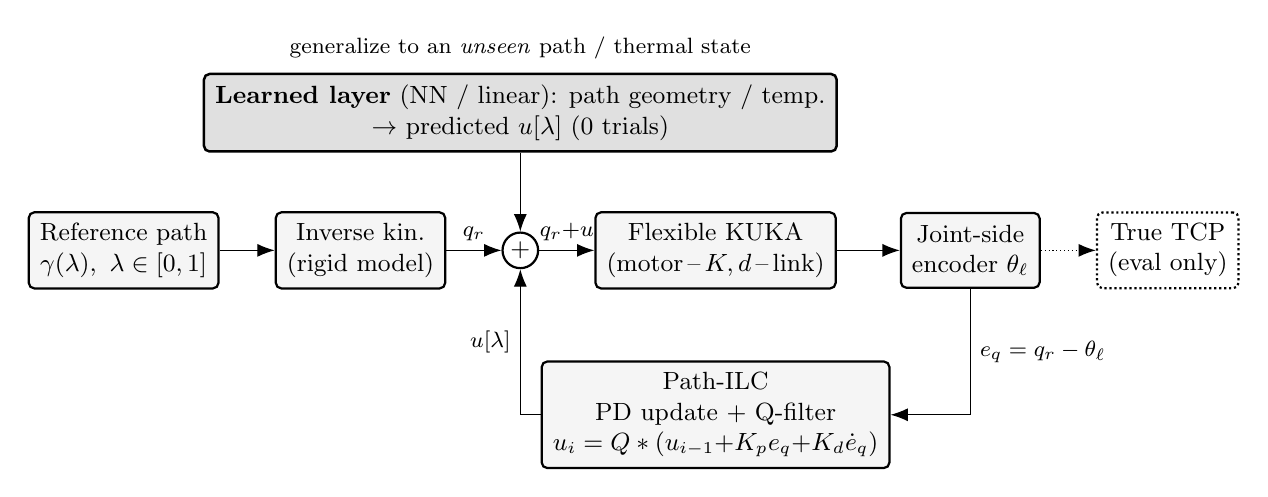
\begin{tikzpicture}[font=\small,>={Latex[length=2.2mm]},
  blk/.style={draw=black,line width=0.8pt,rounded corners=2pt,align=center,minimum height=0.95cm,inner sep=4pt,fill=black!4},
  sum/.style={draw=black,line width=0.8pt,circle,inner sep=1.2pt},
  ai/.style={draw=black,line width=0.9pt,align=center,minimum height=0.95cm,inner sep=4pt,fill=black!12,rounded corners=2pt},
  lab/.style={font=\footnotesize,align=center}]
\node[blk] (ref) {Reference path\\$\gamma(\lambda),\ \lambda\in[0,1]$};
\node[blk,right=0.7cm of ref] (ik) {Inverse kin.\\(rigid model)};
\node[sum,right=0.7cm of ik] (sum) {$+$};
\node[blk,right=0.7cm of sum] (plant) {Flexible KUKA\\(motor\,--\,$K,d$\,--\,link)};
\node[blk,right=0.8cm of plant] (enc) {Joint-side\\encoder $\theta_\ell$};
\node[blk,right=0.7cm of enc,fill=white,densely dotted] (tcp) {True TCP\\(eval only)};
\draw[->] (ref) -- (ik);
\draw[->] (ik) -- node[above,lab]{$q_r$} (sum);
\draw[->] (sum) -- node[above,lab]{$q_r{+}u$} (plant);
\draw[->] (plant) -- (enc);
\draw[->,densely dotted] (enc) -- (tcp);
\node[blk,below=0.9cm of plant] (ilc) {Path-ILC\\PD update $+$ Q-filter\\$u_i=Q*(u_{i-1}{+}K_p e_q{+}K_d\dot e_q)$};
\draw[->] (enc.south) |- (ilc.east) node[pos=0.25,right,lab]{$e_q=q_r-\theta_\ell$};
\draw[->] (ilc.west) -| (sum.south) node[pos=0.75,left,lab]{$u[\lambda]$};
% learned layer centred above the sum -> STRAIGHT vertical arrow
\node[ai,above=1.0cm of sum] (ai) {\textbf{Learned layer} (NN / linear): path geometry / temp.\\$\to$ predicted $u[\lambda]$ (0 trials)};
\draw[->] (ai.south) -- (sum.north);
\node[lab,above=0.05cm of ai] {generalize to an \emph{unseen} path / thermal state};
\end{tikzpicture}
\end{document}
